\section{Calibration through Curve Fitting and Nonlinear Interpolation}

A calibration chart of 256 gray level patches (8-bit) was projected into a flat screen to clearly demonstrate the effects of the inherent gamma of the camera-projector pair in the resulting output image. 
The pixel values from the calibration chart's output image are obtained and compared to the actual values of that of the input. 
The input vs. output (I/O) curve of the camera-projector pair was then derived.
 
From the mean of the subpixels (15x15 pixels) of each cell in the calibration chart, the values for each channel (RGB and grayscale) were plotted as seen in Figure \ref{fig:IO_fit}. It can be observed that the camera-projector pair has a nonlinear (S-shaped) response curve. A polynomial function of the form
\begin{equation}
y = p_1x^4 + p_2x^3 + p_3x^2 + p_4x + p_5,
\label{eq:poly}
\end{equation}
where $p_n (n = 1...5)$ are the parameters for the fitting function, was fitted to the input-output (I/O) curve of the camera-projector pair as observed in Figure \ref{fig:IO_fit}b. 

\captionsetup[figure]{width=5in}
\begin{figure}[h!t]
	\centering
	\subfigure[]{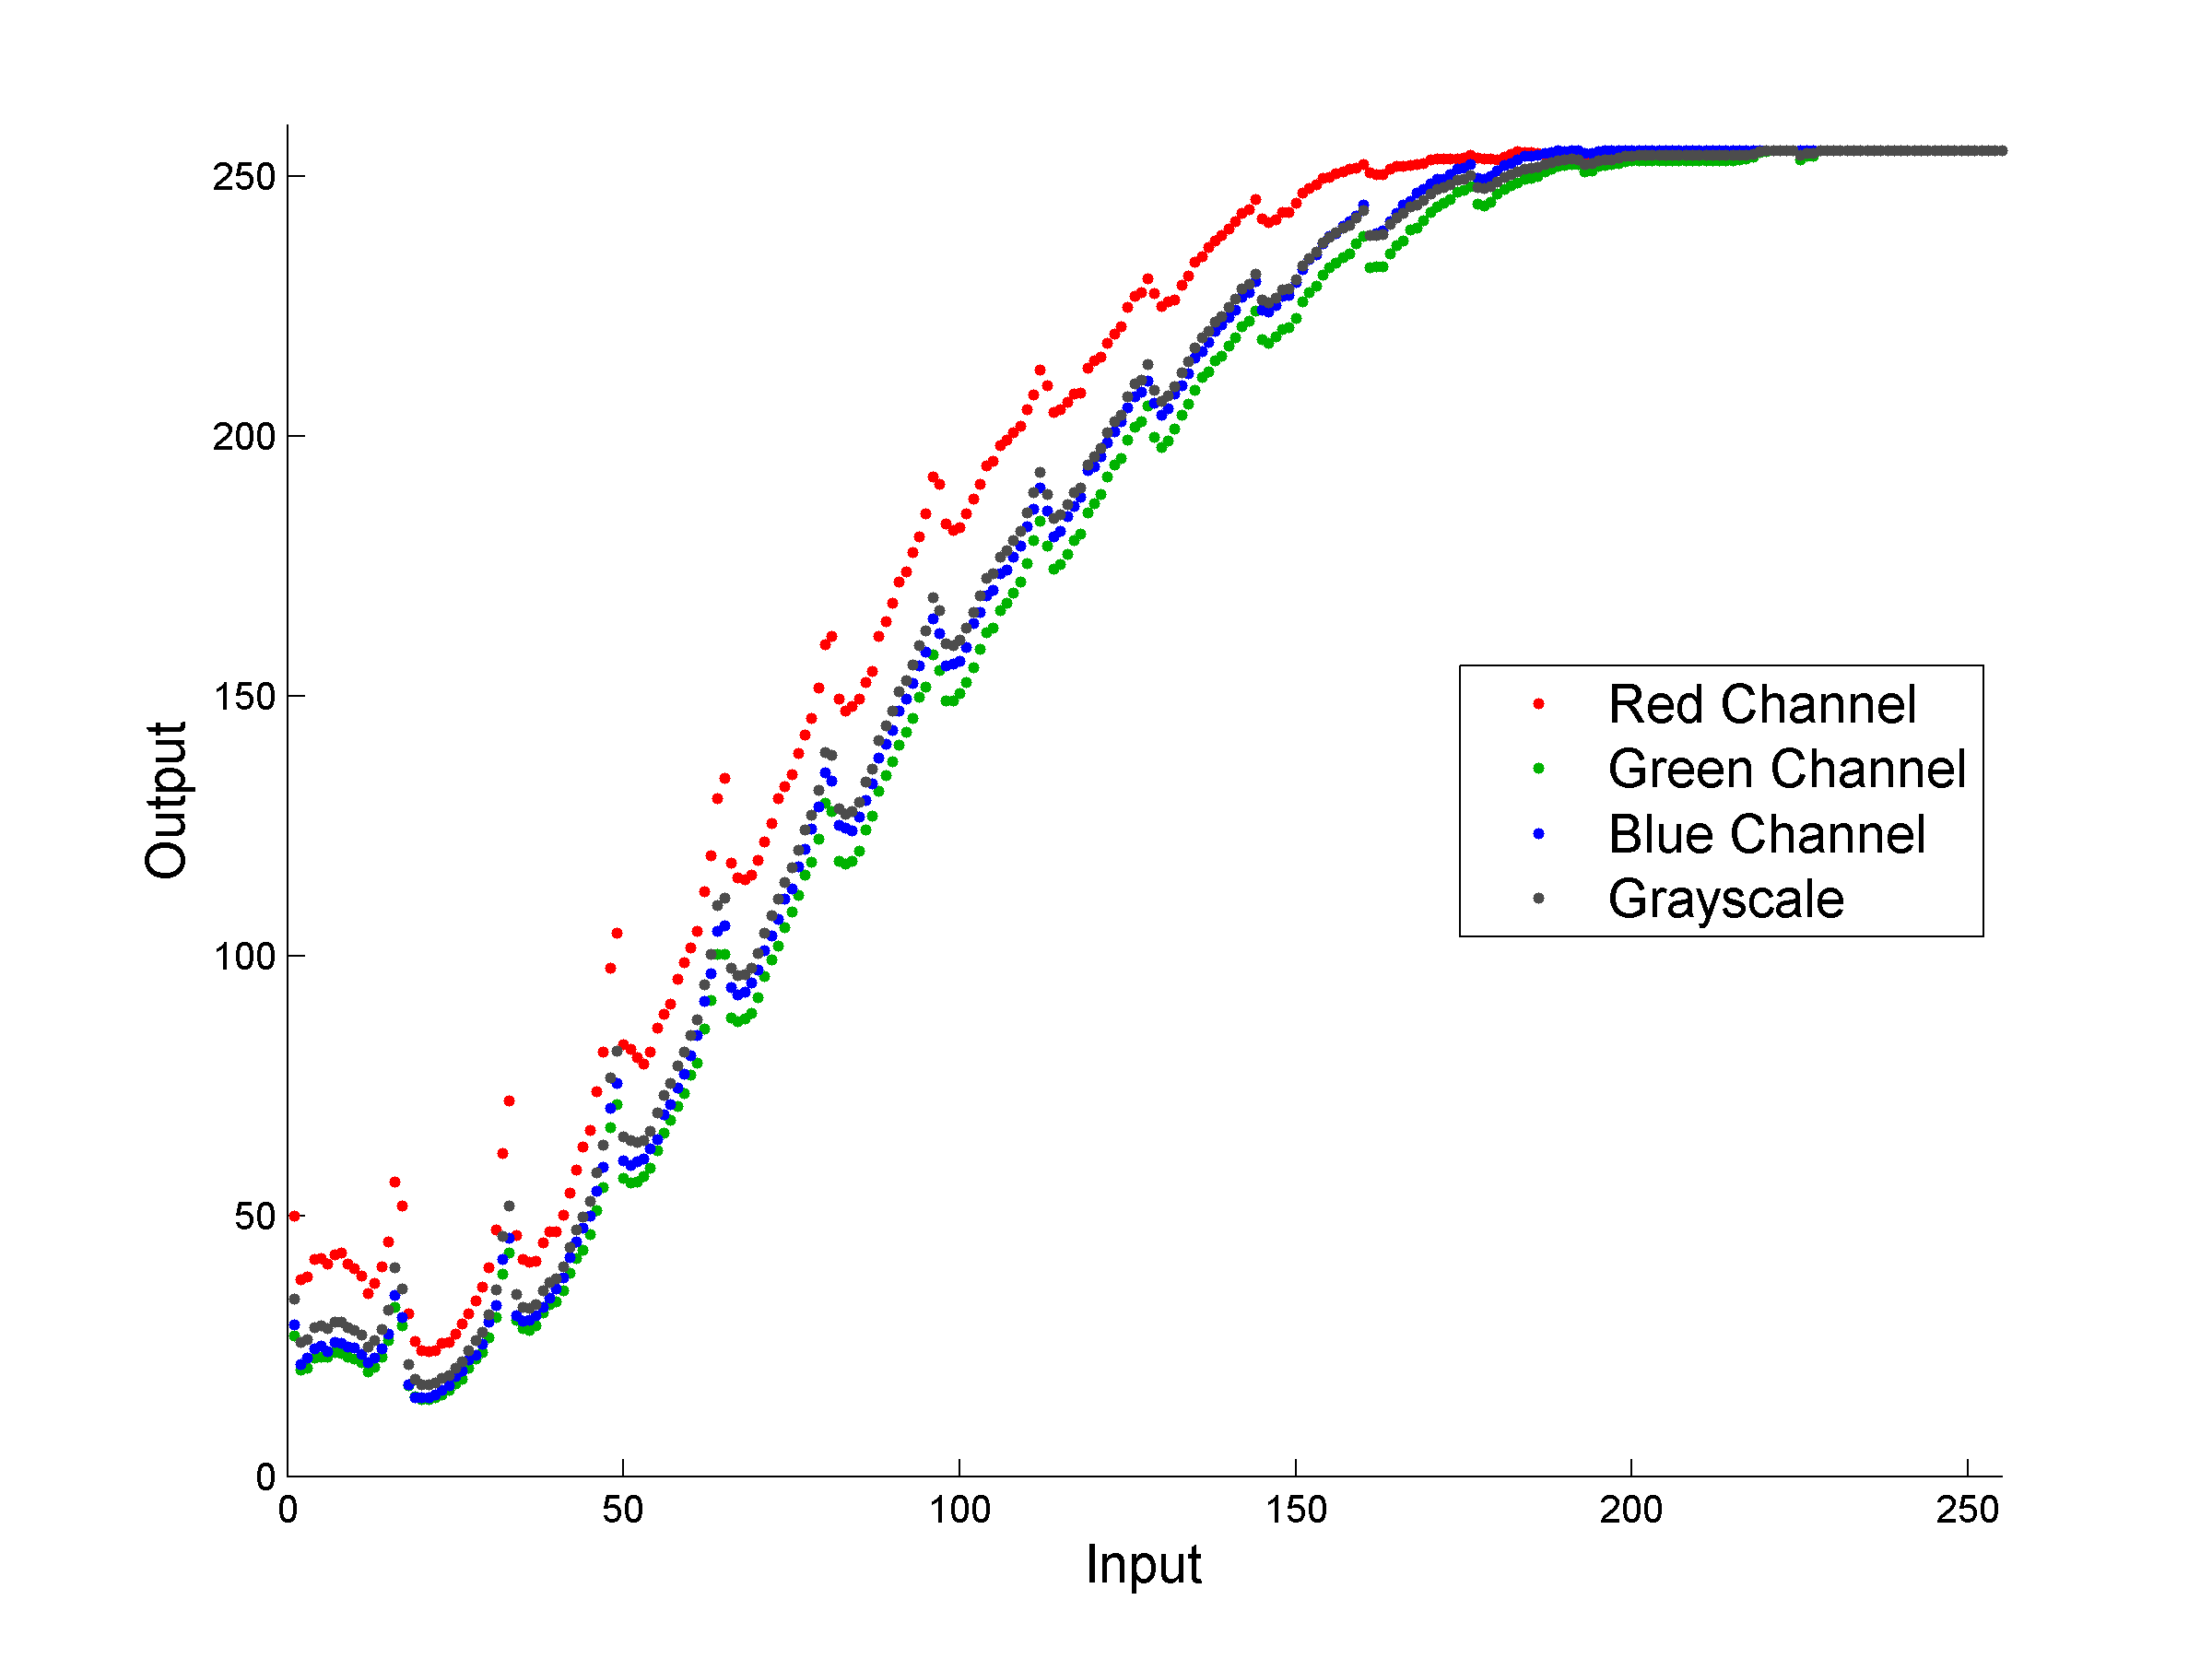
\includegraphics[width=0.475\textwidth]{figures/IOcurve_.png}\label{fig:IO}}
	\subfigure[]{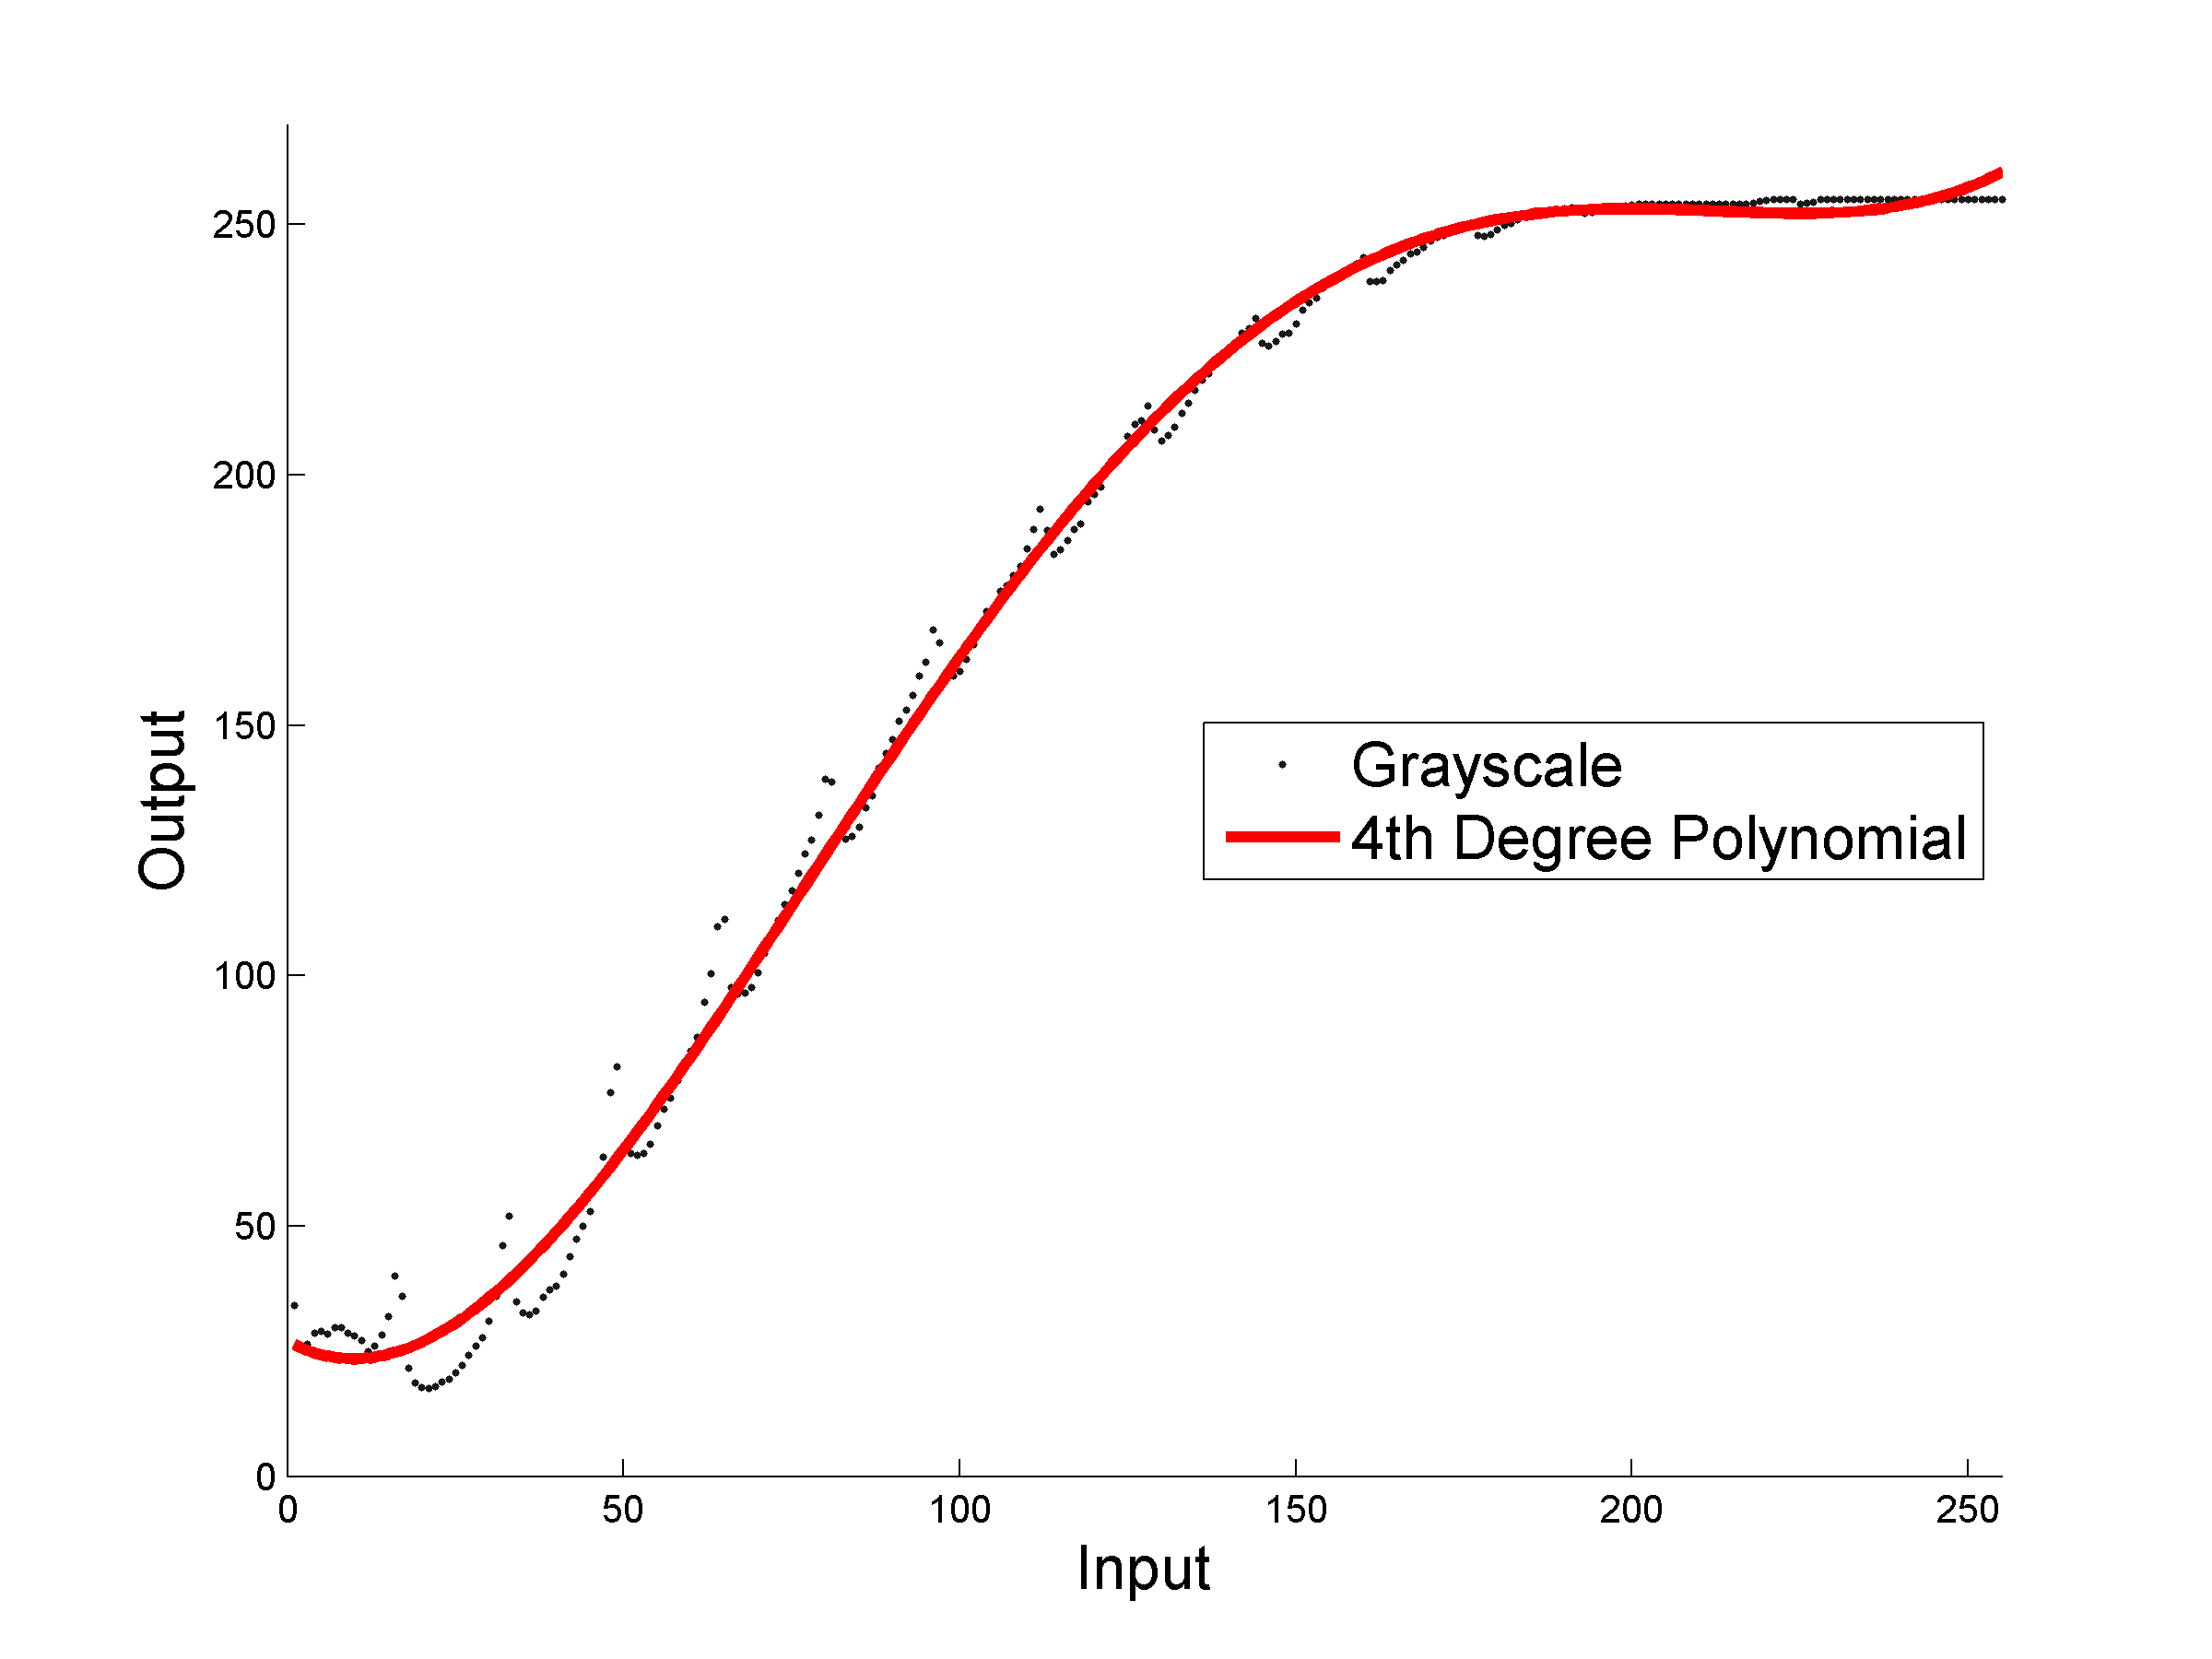
\includegraphics[width=0.475\textwidth]{figures/fits.png}\label{fig:fit}}
	\caption[Input-output curve of the calibration chart]{\subref{fig:IO} I/O curve of the grayscale and RGB channels of each pixel value in the calibration chart and (b) the 4th degree polynomial function fitted to the grayscale using nonlinear fitting.}
	\label{fig:IO_fit}
\end{figure}

The 4th degree polynomial function served as the basis for the nonlinear fitting since if we dissect each term in it, e.g. we look at the first term, $x^4$, we will see that it already is a power function which obeys the form of our gamma. The dark current of the system that we see as the noisy signal at the lower values of the I/O curve, the analog-to-digital conversion (ADC) which is seen as the saturation in the upper limits of the curve, as well as the constant shift all have contributions to the form of the curve and each takes up a term in the function. All the terms combined already takes into account the gamma of the whole PSP system. 

Moreover, the 4th degree polynomial function gives the least number of residuals among the high-order polynomial functions. A cubic spline and a sigmoid function were also fitted to the I/O curve but the 4th degree polynomial function still gave the best fit. 

The obtained parameters for $p_n$ were $p_1 = 3.41$, $p_2 = -0.000153$, $p_3 = 0.0129$, $p_4 = 1.95$, and $p_5 = 22.8$. Without considering the constant, $p_5$, we observe that the highest $p$ factor is that of $p_1$, also having the greatest contribution to the form of the curve. These parameters, however, are for the camera and projector combined and so, we cannot really pinpoint which equipment has the greater contribution for these factors. Nevertheless, what we are interested in is the calibration of the whole system and not the individual equipment.

By knowing the actual input (0 to 255) and the polynomial function with the correct parameters, the inverse function was finally obtained via interpolation.
\captionsetup[figure]{width=5in}
\begin{figure}[h!t]
	\centering
	\subfigure[]{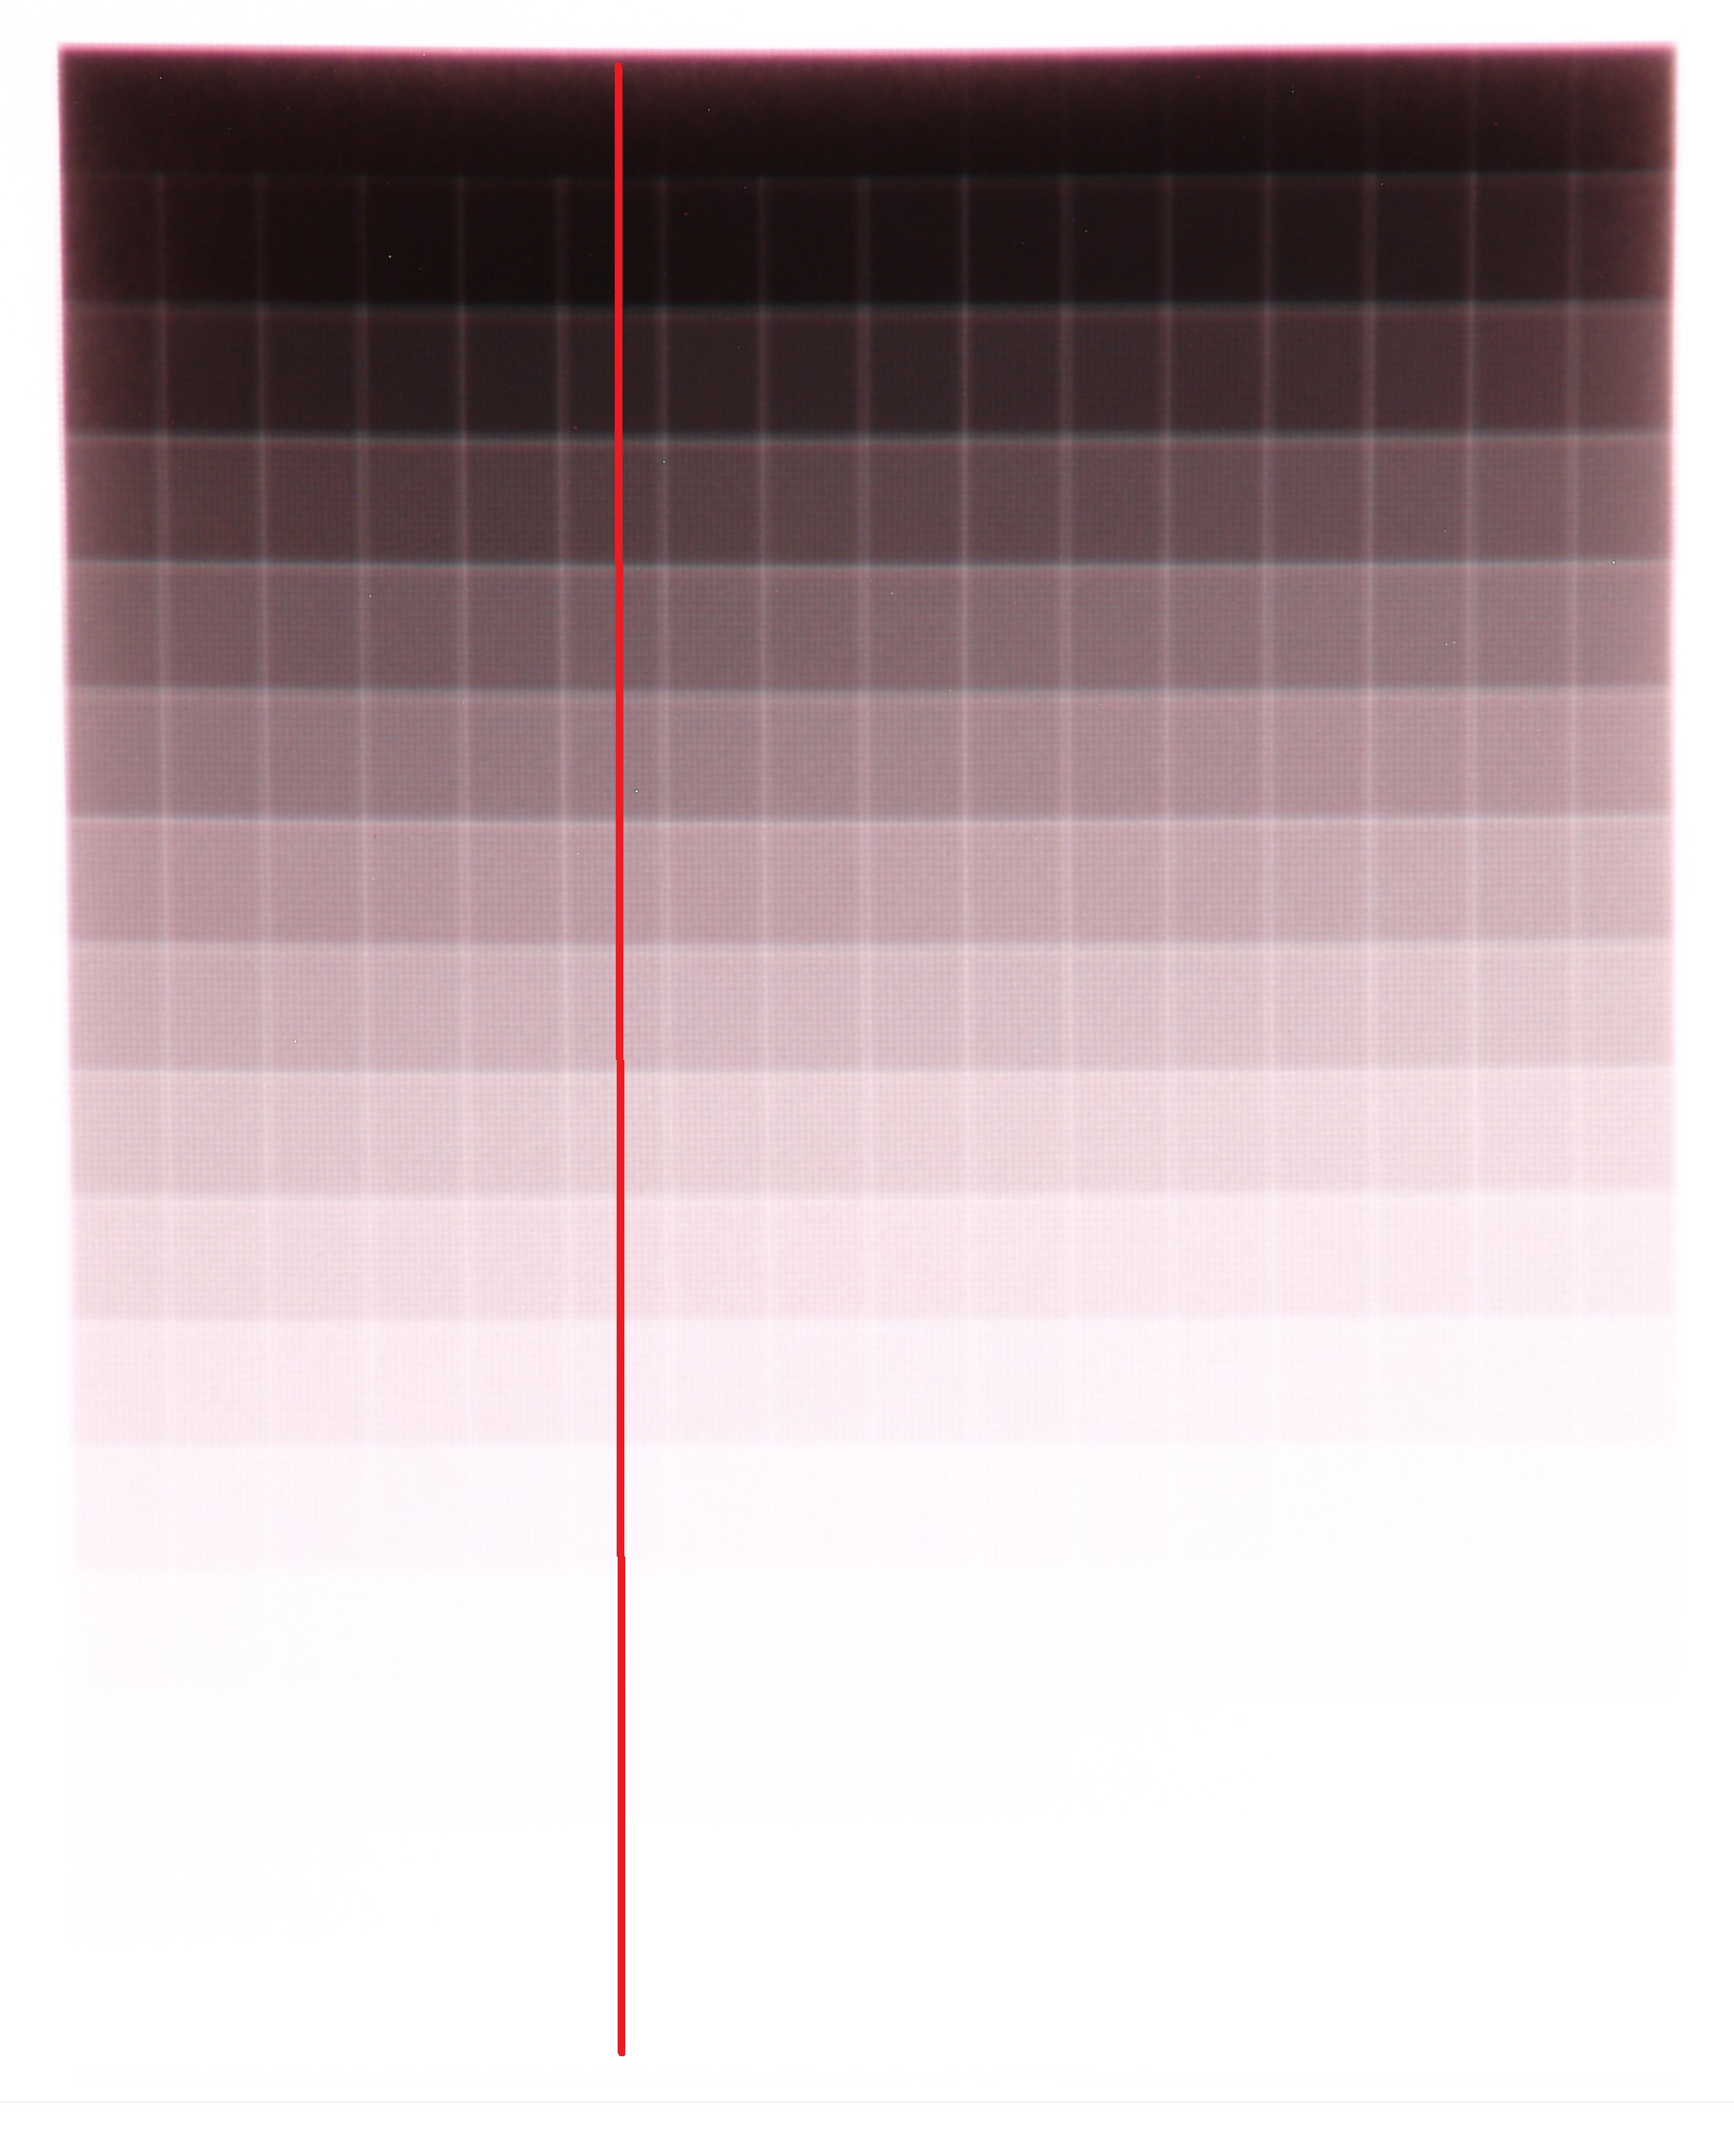
\includegraphics[height=0.35\textwidth]{figures/grid.jpg}\label{fig:input_calib}}
	\subfigure[]{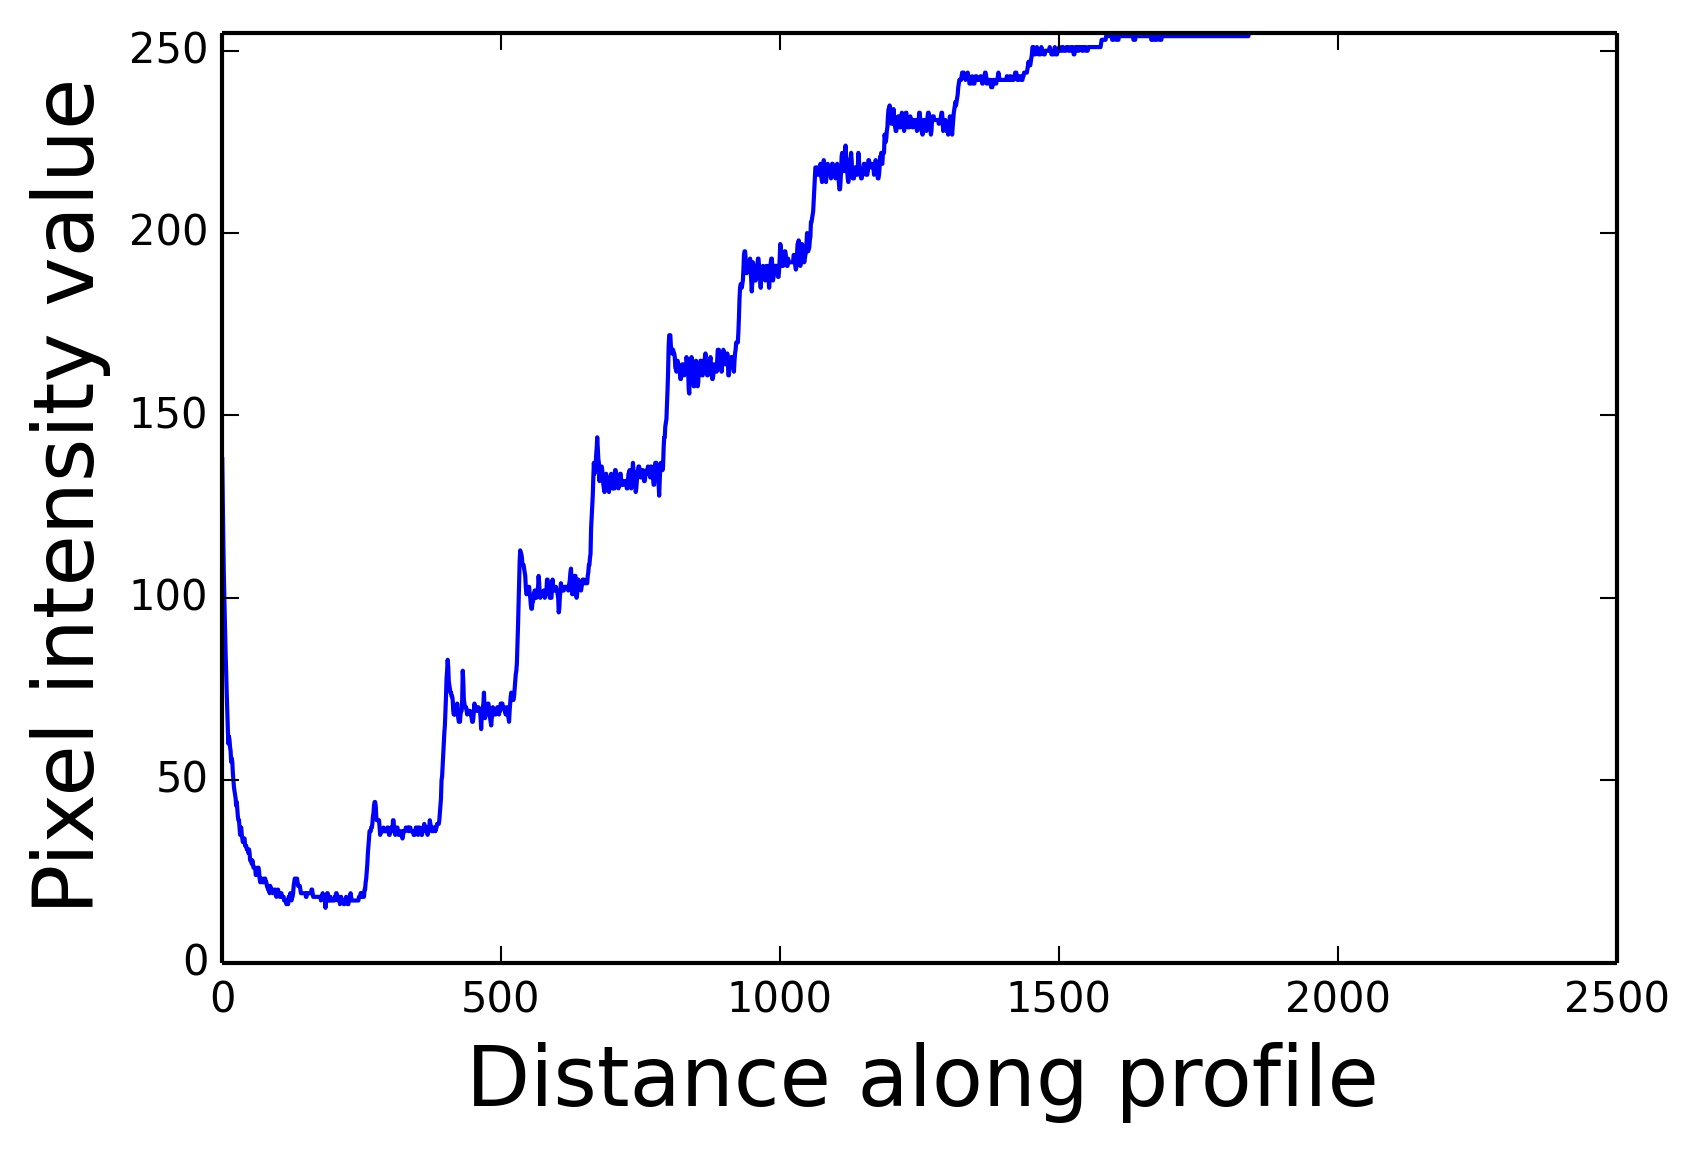
\includegraphics[height=0.35\textwidth]{figures/g_profile.jpg}\label{fig:input_profile}}
	\subfigure[]{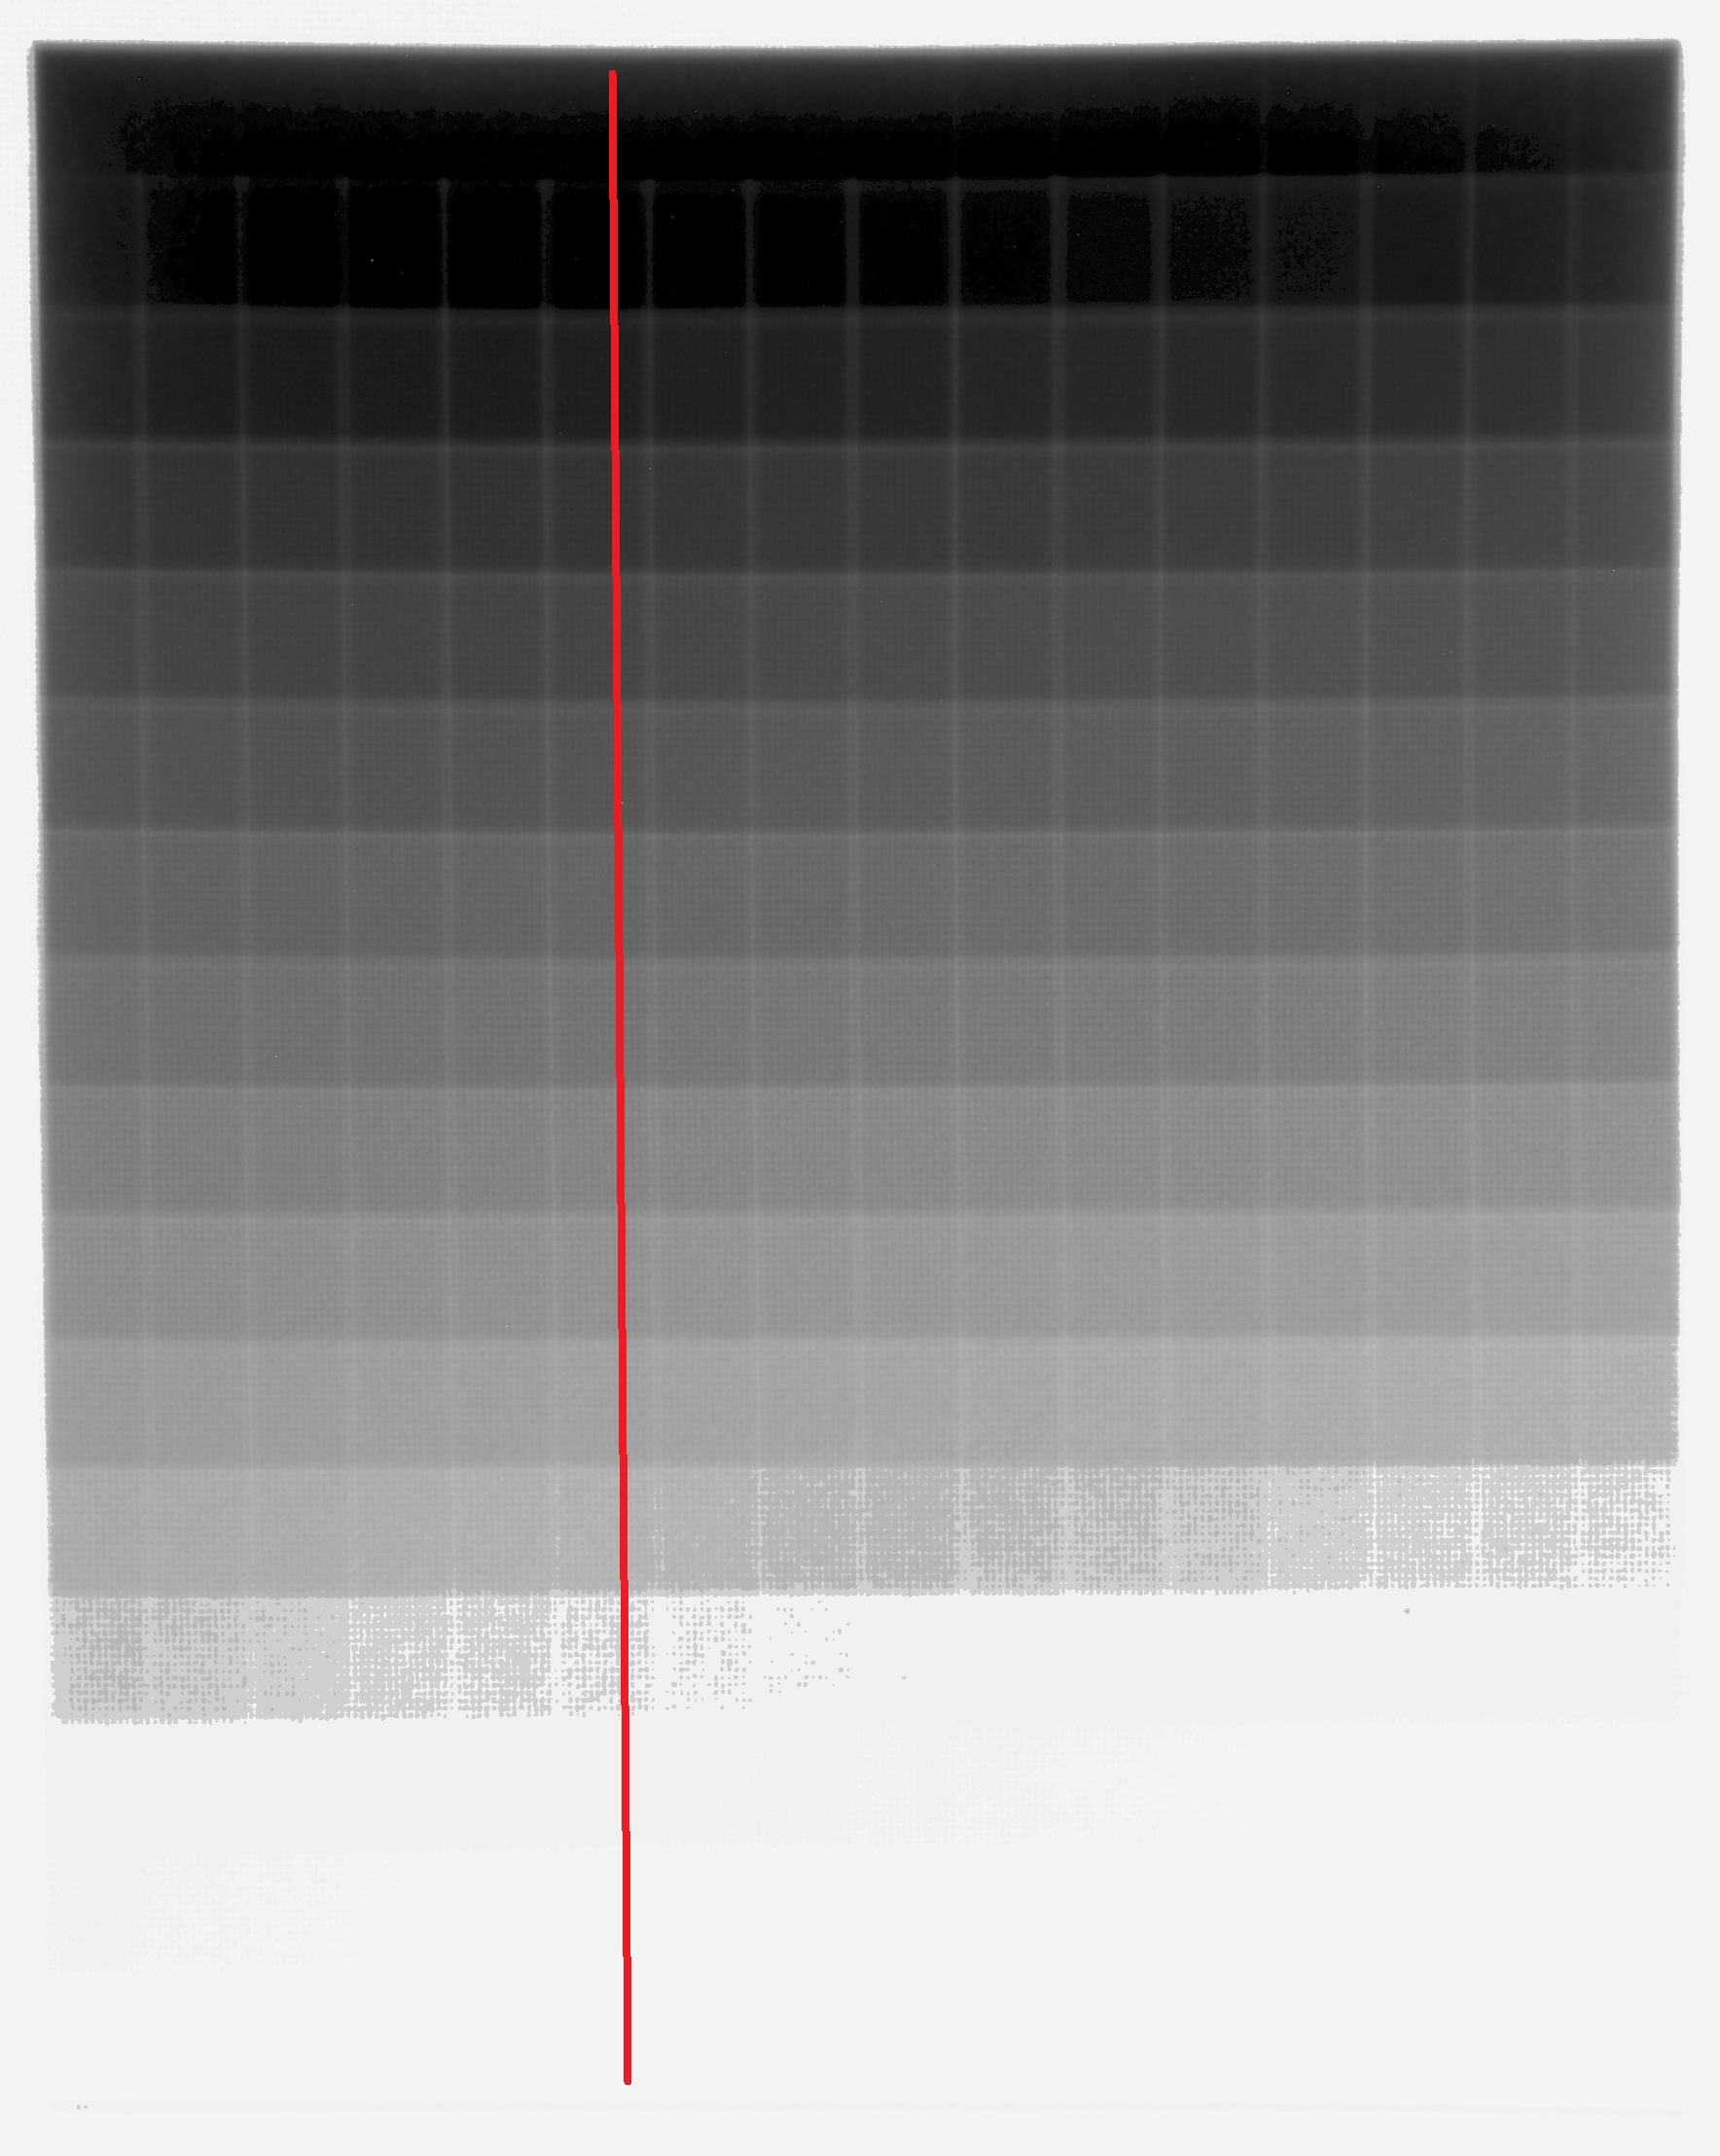
\includegraphics[height=0.35\textwidth]{figures/linear.jpg}\label{fig:linear_calib}}
	\subfigure[]{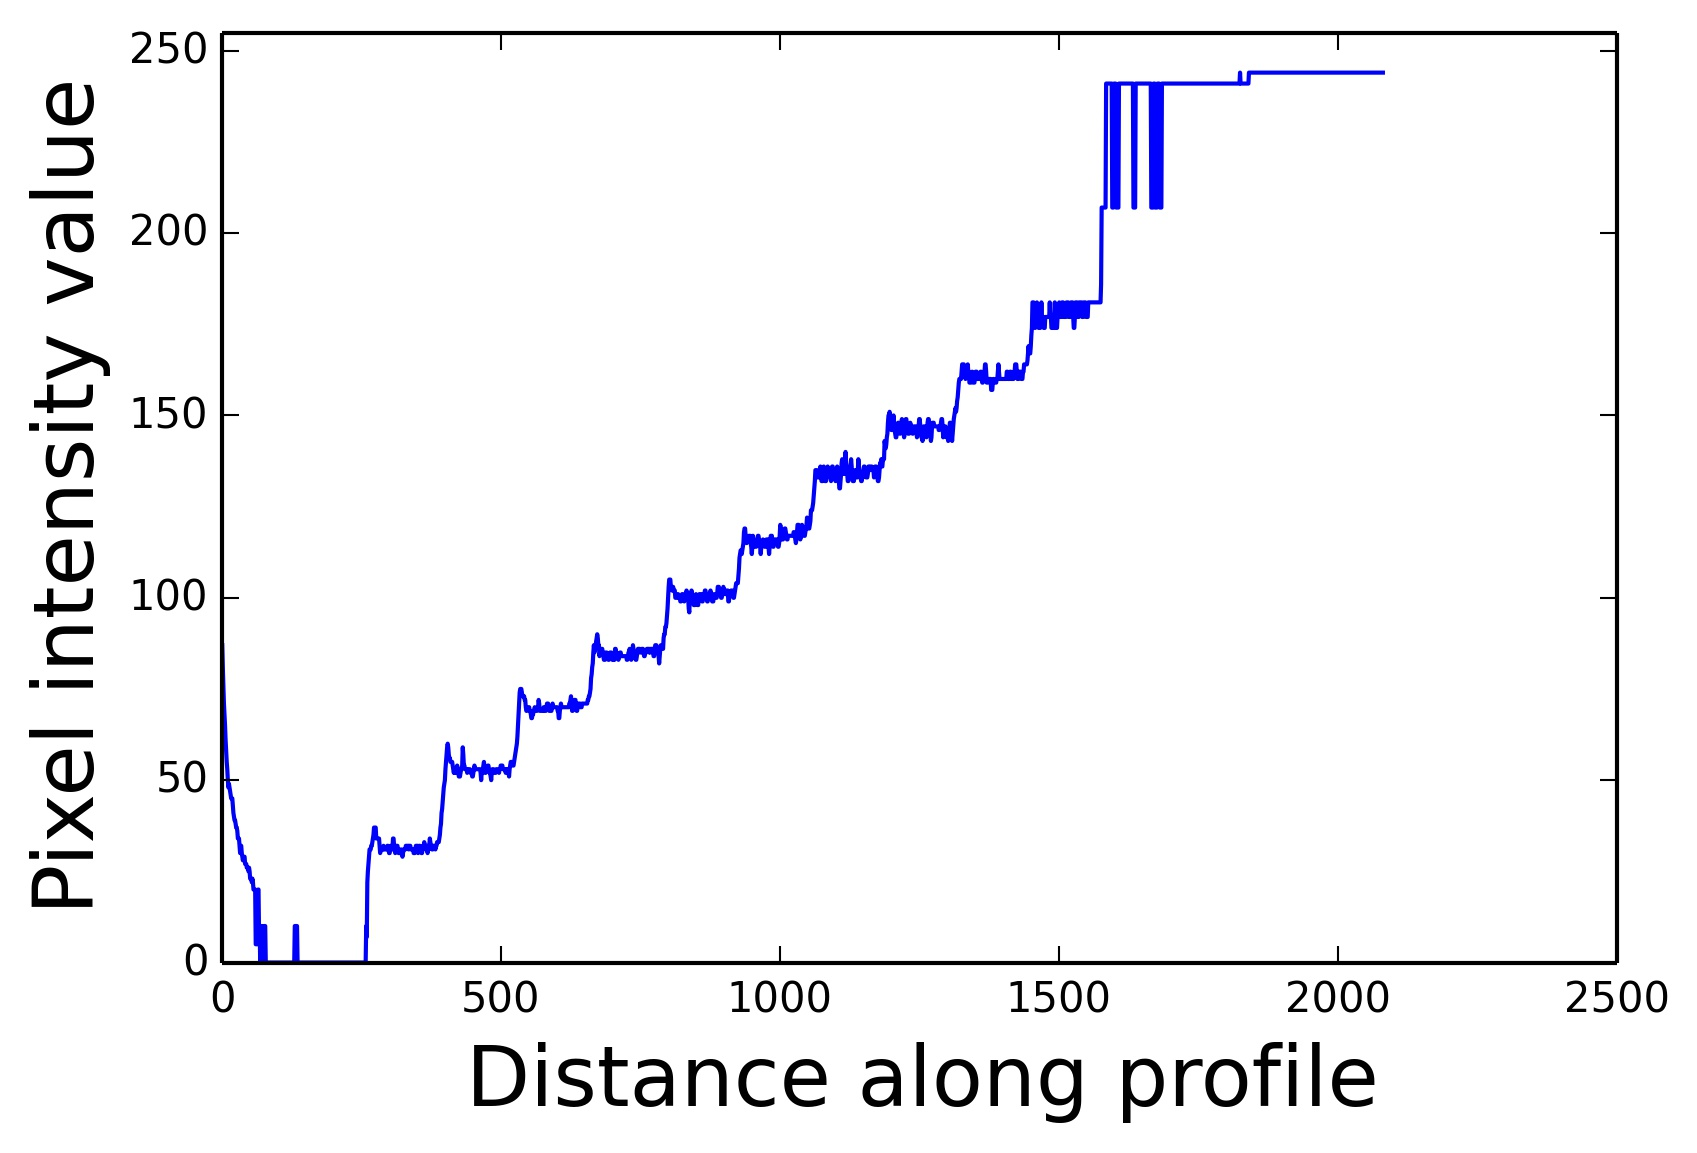
\includegraphics[height=0.35\textwidth]{figures/l_profile.jpg}\label{fig:linear_profile}}
	\caption[Nonlinearized and linearized calibration charts and intensity profiles]{Calibration charts and intensity profiles (red lines): \subref{fig:input_calib} Output image and
		\subref{fig:input_profile} its intensity profile
		\subref{fig:linear_calib} Linearized output image and 
		\subref{fig:linear_profile} its intensity profile}
	\label{fig:calib}
\end{figure}

Intensity profiles of the nonlinearized and linearized output images of the calibration chart were taken to verify the effect of the linearization. 

From Figure \ref{fig:calib}, the difference in the intensity profiles are indeed visible as that of the output image takes the form of the S-shaped curve. Upon linearization, it was observed that the most linearized parts of the ouput image are the pixel values greater than 50 and less than 200, based from the intensity profile in Figure \ref{fig:calib}d. 

We notice that the high-intensity values are obscured in the linearized calibration chart (see Fig. \ref{fig:calib}c). This is due to the camera setting used wherein the exposure time of 2.5 s resulted to a high level of intensity of the overall image or a saturation, making these values hard to linearize. The high-intensity values of the linearized calibration chart had a noisy data. 

\section{Gamma Inversion Application in Fringe Intensity Biasing}
Projected fringes were initially created using a sinusoidal wave along the x-direction having the following equation:
\begin{equation}
\textrm{fringe} = I_o(\sin(2\pi f t + n\phi))
\label{sine wave}
\end{equation}
where $I_o$ is the relative intensity of the fringe set to 0.25, $f$ is the frequency set to 40 Hz, $t$ is time set to 1500 seconds, $n$ is the fringe number (1 to 4), and $\phi$ is the phase shift which was set to $\pi/2$ or 90$^o$ resulting to four fringes with phase shifts of 0$^o$, 90$^o$, 180$^o$, and 270$^o$.

\captionsetup[figure]{width=5in}
\begin{figure}[h!]
	\centering
	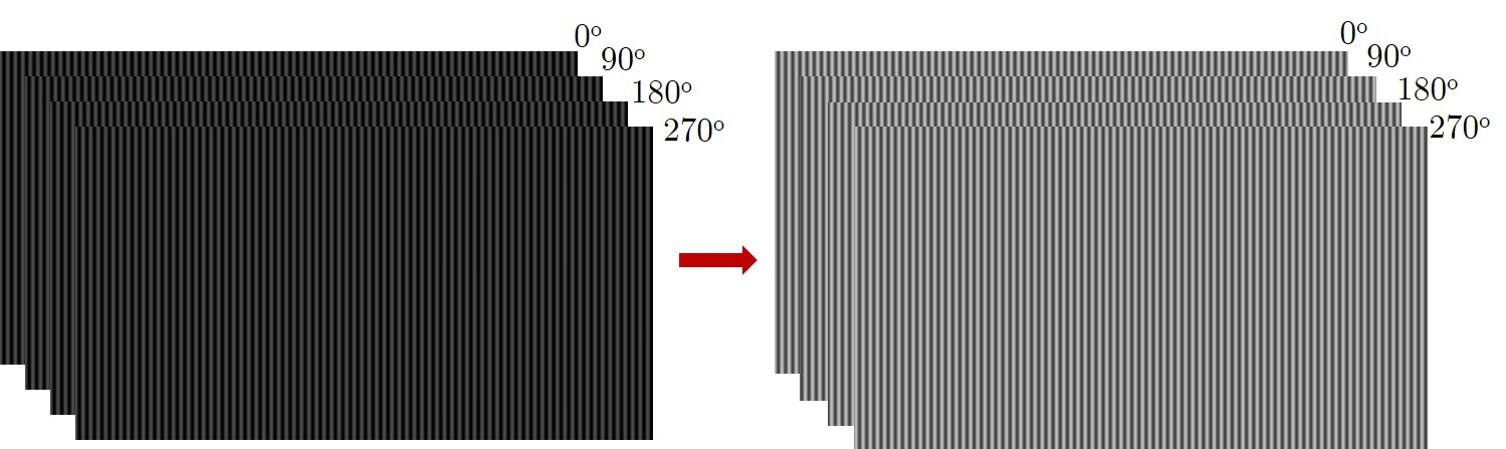
\includegraphics[width=1\textwidth]{figures/fringes.jpg}
	\caption[Fringes before and after gamma inversion]{Fringes before (left) and after intensity biasing (right).}
	\label{fig:fringes}
\end{figure}

Based from the result of linearization, a biasing of the intensity of the fringes was implemented to get better quality 2D images for the 3D reconstruction.
The obtained polynomial curve was fitted to the original fringe.

A constant was simply added to the sine wave equation but with the other parameters retained resulting to the following modified equation: 

\begin{equation}
\textrm{fringe}_\textrm{biased} = I_o(\sin(2\pi f t + n\phi) + 2)
\end{equation}

This constant simply shifts the intensity of the projected fringes to a higher minimum and maximum that is within the most linearized range ($>50$ and $<200$) of the camera-projector pair.

Since sine functions have limits of [-1,1], adding the constant 2 will shift the limits to [1,3] and multiplying each to 0.25*255 (0.25 for the set intensity and 255 for the highest grayscale level\footnote{Note that we are operating on grayscale images}), then we have a biased fringe intensity of [63.75,191.25] from [-63.75,63.75].

Figure \ref{fig:fringes} shows the image of the original fringe and the change in the intensity level of the fringes upon application of intensity biasing.

As for the frequency of the fringes, it was observed that the higher the set of the frequency of the fringes are, the finer the details of the reconstructions will be.

Gamma inversion/correction need not be done several times for a particular camera-projector pair once the fringes are biased to fit the linear range. Changes in the form of the polynomial curve for different camera settings were found to only have shifts for the constant part (p5) but the shape of the curve remains the same. 
